\section{Validation Results}

In this section, we will go through each validation scenario discussed in \autoref{ch3:validation_roadmap}. We will review the output, but not all output figures are included here. For a complete set of images, refer to \autoref{appendix_b}.

\subsection{Most Recent Contributor}
It shows the contributor who made the most recent changes to the method. To achieve this, we extracted methods and authors as nodes.

The expected output for this probe is a method node containing detailed information about the method. This node should be linked to author nodes, representing all contributors who have modified the method. Among these connections, a relation should indicate the most recent contributor, determined by the latest modification date.

Instead of displaying all methods and their authors (which can be viewed in the \autoref{appendix_b}), we will take one method as an example and present its results.

We can use Neo4j Cypher queries\footnote{\url{https://neo4j.com/docs/cypher-manual/current/queries/}} to filter and retrieve the required data.

\begin{lstlisting}[language=SQL]
MATCH (n)-[r]-(m)
WHERE n.signature = "org.springframework.samples.petclinic.customers.web.OwnerResource.createOwner(org.springframework.samples.petclinic.customers.web.OwnerRequest)"
RETURN n, r, m
\end{lstlisting}

This will extract information only about the method based on our probe settings and the output JSON. After displaying the results in the visualizer, we can further interact with the nodes and edges in the Neo4j browser to explore additional relationships.

\begin{figure}[ht]
    \centering
    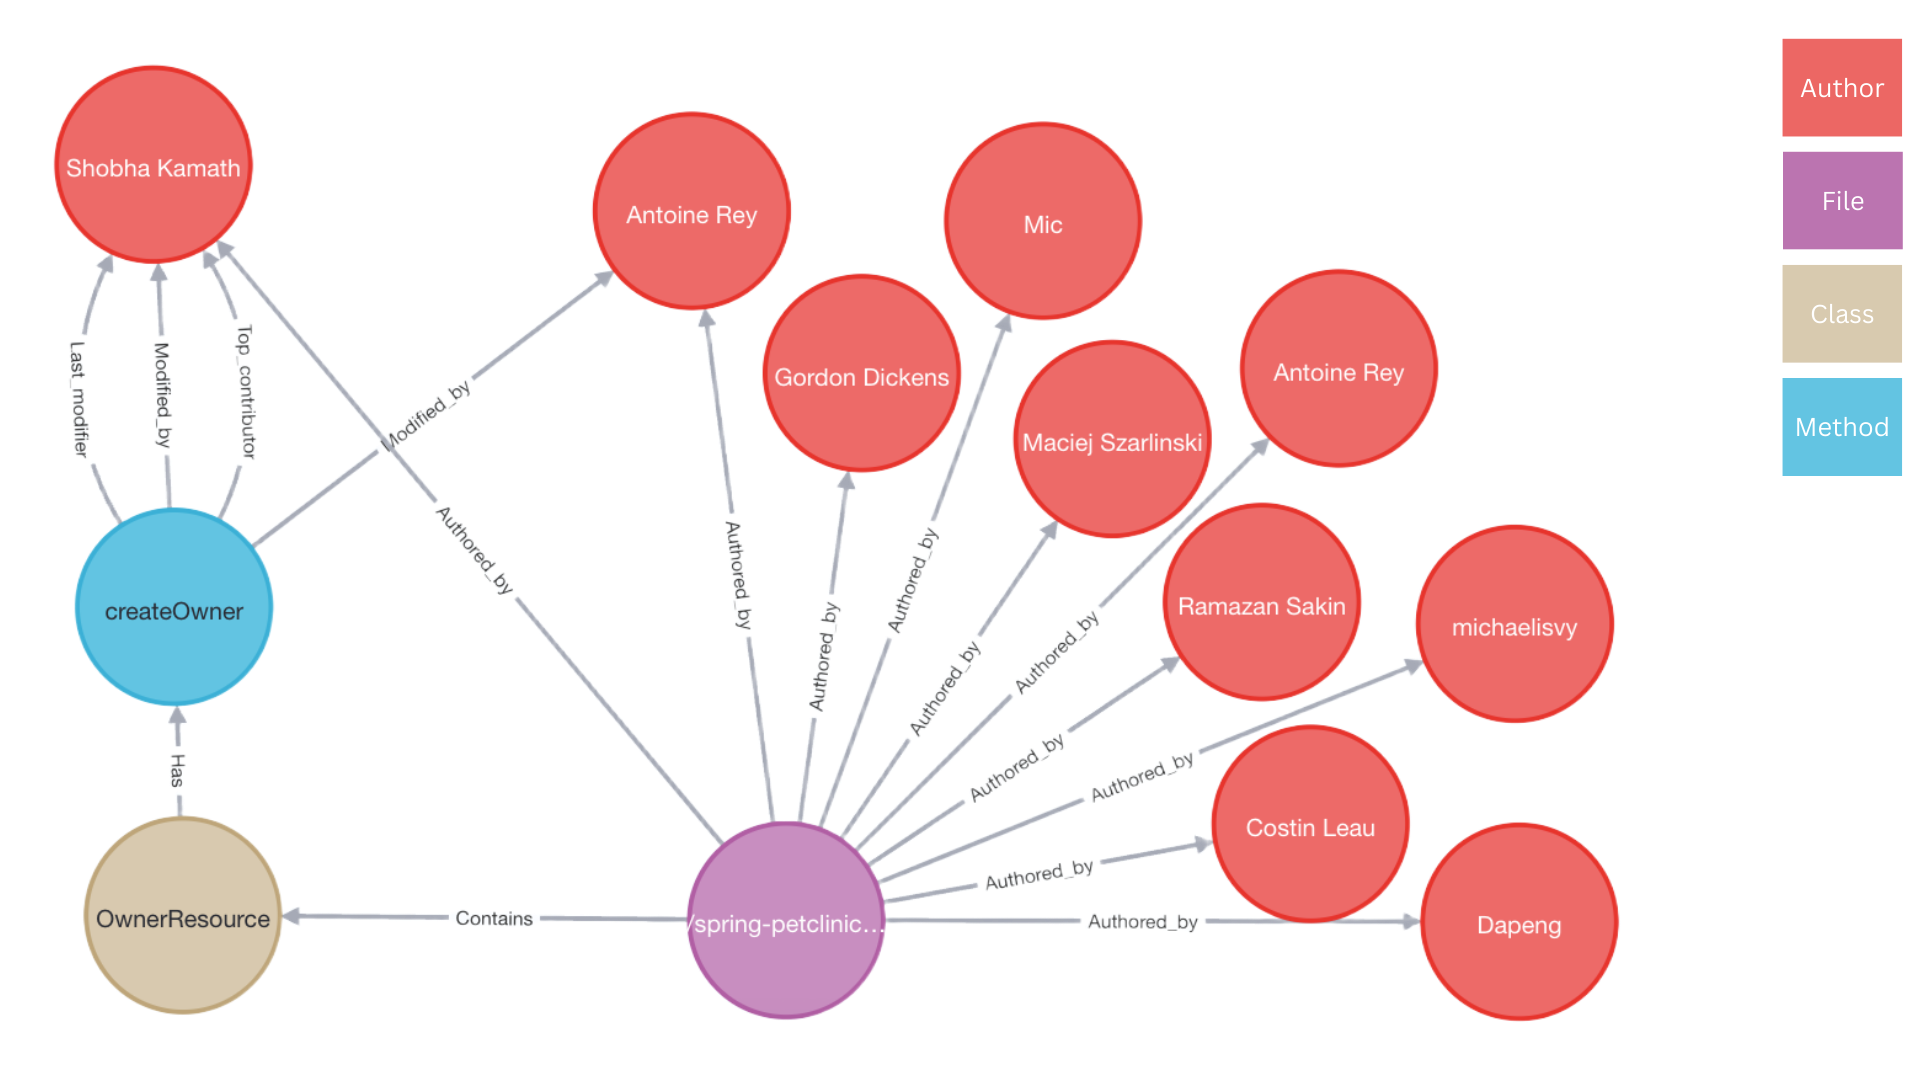
\includegraphics[width=0.9\textwidth]{figures/author_file_class_method_relation.png}
    \caption{Neo4j Browser showing the relation between nodes}
    \label{fig:scenerio_1_2_3_overview}
\end{figure}

\autoref{fig:scenerio_1_2_3_overview} illustrates the node relationships in the Neo4j Browser visualizer. We have used the query mentioned above to extract the data and extend class and file relations.\ Additional data and details can be included in each relationship edge. For example, the \texttt{Last\_modifier} relationship displays the last modification date and time.

\subsection{List of Contributors}
It shows all the contributors of the methods. The expected output for this probe is a set of author nodes and methods.

\autoref{fig:scenerio_1_2_3_overview} illustrates two authors who modified the \texttt{createOwner} method. The author nodes contain information about the authors, such as their names and email addresses, while the method nodes store details about the method, including a unique identifier. In the current probes, we uniquely identify a method by combining the package name of the Java file, the class name, and the method signature. Authors are identified using their email addresses, as multiple contributors may have the same name, but email addresses are always unique.

\subsection{Top Contributor}
It identifies the top contributor to the method. Instead of creating a separate node for the top contributor, we establish a relationship edge from the method node to the author node, labeled as \texttt{Top\_contributor}. This relationship includes properties that indicate the total lines added by the top contributor, along with the specific code line numbers of their contributions.

\autoref{fig:scenerio_1_2_3_overview} illustrates two authors who modified the method \texttt{createOwner}. Among them, the author \textit{Shobha Kamath} has a \texttt{Top\_contributor} relationship edge attached, indicating that they are the top contributors to this method.

\subsection{File Contributors}
It displays the list of contributors for each file. To achieve this, we extracted files and authors as nodes. Like the top contributor approach, we represent file authorship by establishing a direct relationship between files and authors. An edge from a file node to an author node, labeled as \texttt{Authored\_by}, indicates that that particular contributor authored the file.

\autoref{fig:scenerio_1_2_3_overview} illustrates all the current authors of the file.

\subsection{Author Relation}
It represents the joint contributions between two authors, measured by the number of file collaborations. The strength of the connection between the two authors indicates the number of shared contributions.

We can show this by connecting the names of two authors to the \texttt{Author\_Relation} node. This node contains data such as the strength of their collaboration and a list of files they have worked on together.

Since this analysis is more statistical, we can visualize it using \textit{Tableau}. \autoref{fig:scenerio_1_2_3_overview} illustrates the relationship strength between authors. The highlighted section shows an example of a quantitative connection between two contributors. Further analysis can be performed based on specific requirements, such as sorting by increasing contribution strength or integrating the data into an organization's dashboard to visualize team collaboration.

\begin{figure}[H]
    \centering
    \rotatebox{-90}{
        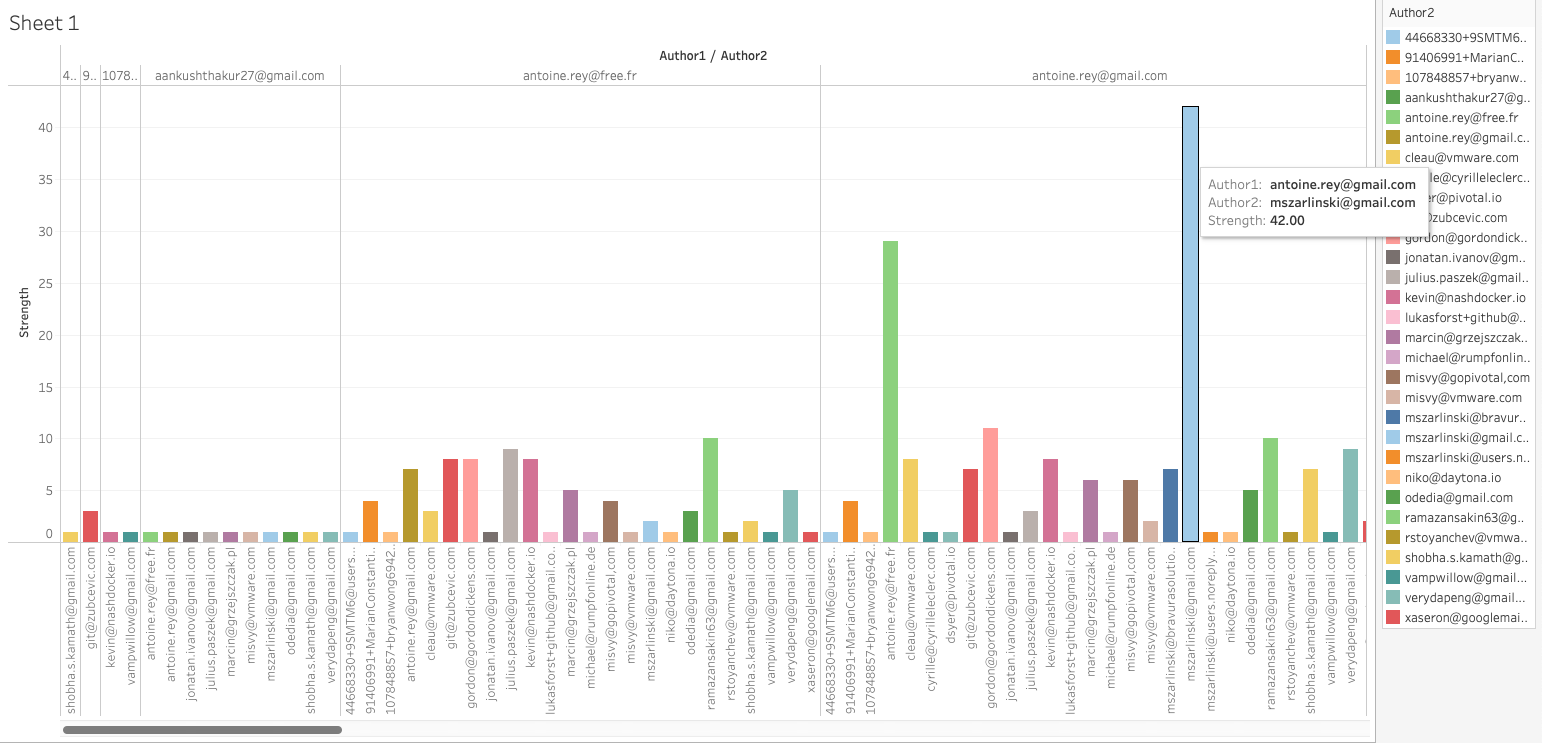
\includegraphics[height=0.6\linewidth]{figures/author_relation_strength.png}
    }
    \caption{Tableau tool showing authors' relation strength}
    \label{fig:auth_relation_strength}
\end{figure}


\subsection{REST API Endpoints}
It displays all the REST API endpoints in the project. Methods and endpoints were extracted as nodes using a Cypher query.

\begin{lstlisting}[language=SQL]
MATCH (a)-[r]-(b)
WHERE type(r)="Maps"
AND a.name="PetResource"
RETURN a, r, b
\end{lstlisting}

The expected output should include class and endpoint nodes. Each class should be connected to its corresponding endpoint nodes using a \texttt{Maps} relationship, as a class maps REST API endpoints.

\autoref{fig:file_class_endpoint} illustrates a class node, \texttt{PetResource}, mapping four endpoints. The file node shown in the figure was not extracted from the initial query. Instead, it was obtained using the Neo4j Browser node relationship extractor after executing the query.

\begin{figure}[H]
    \centering
    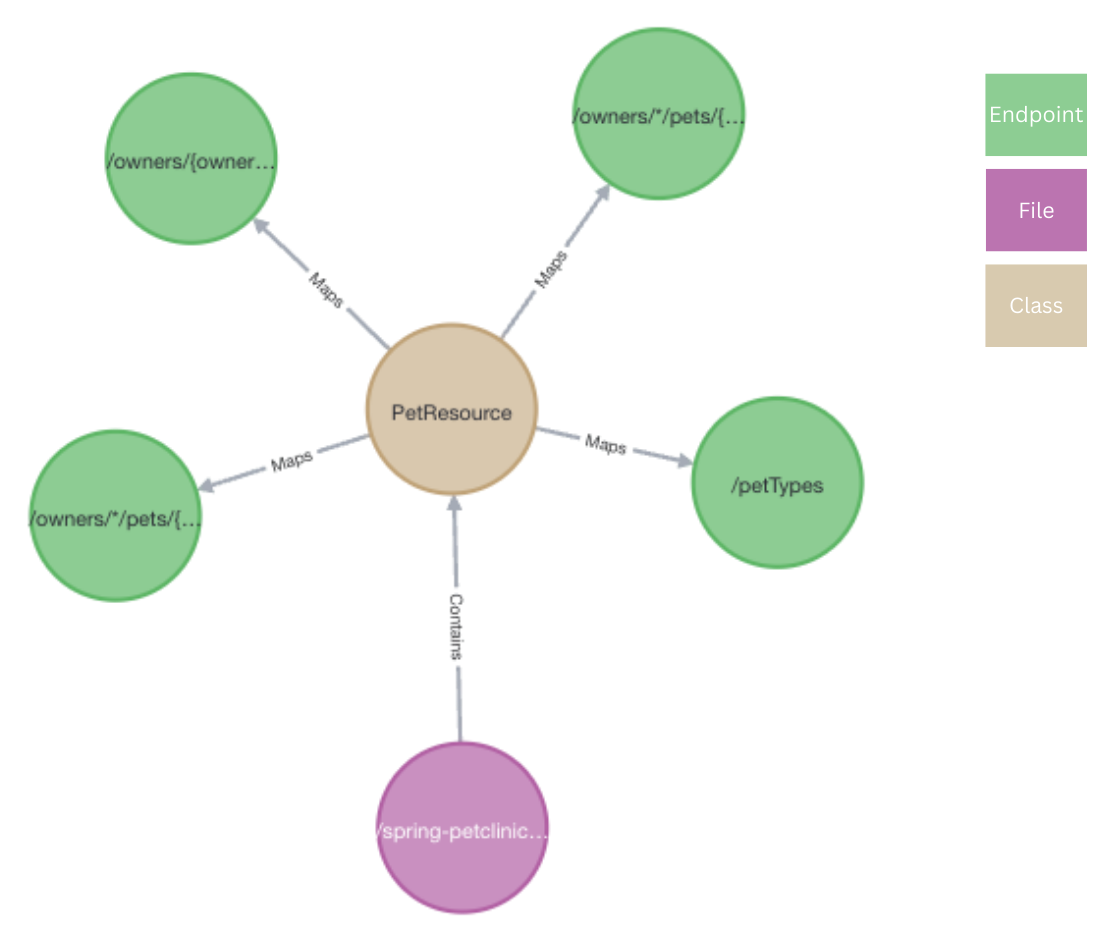
\includegraphics[width=0.6\textwidth]{figures/file_class_endpoint.png}
    \caption{Neo4j Browser showing the relation between class and REST API endpoints}
    \label{fig:file_class_endpoint}
\end{figure}

\subsection{Java Beans}
It identifies Java Spring bean classes and methods. To achieve this, we extract files, classes, and methods. The expected output includes a file node that has a \texttt{has\_bean\_class} relationship with a class identified as a candidate bean class. This bean class, in turn, has a \texttt{has\_bean\_method} relationship with methods that are considered candidate bean methods.

\subsection{Dependencies List}
It displays all the Maven project dependencies in the project. To achieve this, we locate the \textit{Project Object Model (POM)} file and parse its dependencies.

The expected output consists of a POM file node and multiple dependency nodes. Each dependency contains metadata such as version and scope. Dependencies are identified using their \texttt{artifact\_id} and \texttt{group\_id}.

The POM file node is connected to the dependency nodes through a \texttt{depends\_on} relationship.